\documentclass[a4paper]{article}
\usepackage[UTF8]{ctex}
\usepackage{geometry}
\usepackage{graphicx}
\usepackage{url}
\usepackage{multirow}
\usepackage{array}
\usepackage{booktabs}
\usepackage{url}
\usepackage{enumitem}
\usepackage{graphicx}
\usepackage{float}
\usepackage{amssymb}
\usepackage{amsmath}
\usepackage{subfig}
\usepackage{longtable}
\usepackage{pifont}
\usepackage{color}

\allowdisplaybreaks

\geometry{a4paper, scale=0.78}

% \begin{figure}[H]
%     \centering
%     \includegraphics[width=.55\textwidth]{E.png}
%     \caption{矩阵与列向量的乘法}
%     \label{fig:my_label_1}
% \end{figure}

% \left\{
% \begin{array}{ll}
%       x+2x+z=2 & \\
%       3x+8y+z=12 & \\
%       4y+z=2
% \end{array}
% \right.

% \begin{enumerate}[itemindent = 1em, itemsep = 0.4pt, parsep=0.5pt, topsep = 0.5pt]

% \end{enumerate}

%\stackrel{a}{\longrightarrow}

%\underbrace{}_{} %下括号

%\tableofcontents %目录,并且目录页不记录页码
% \tableofcontents
% \newpage
% \setcounter{page}{1} %new page
% \clearpage

\title{Spectral Clustering}
\author{Chen Gong}
\date{02 March 2020}

\begin{document}
\maketitle
%\pagestyle{empty}
\tableofcontents
\newpage
%\pagestyle{fancy}
\setcounter{page}{1} %new page
\clearpage

\section{Background}
本章节主要是描述的一种聚类算法,谱聚类(Spectral Clustering)。对机器学习有点了解的同学对聚类算法肯定是很熟悉的,那么谱聚类和之前普通的聚类算法有什么不一样呢?或者说它有什么优势呢?

\subsection{聚合型聚类(Compactness)}
常见的聚类方法有两种思路,一种就是聚合型聚类(Compactness)。典型的算法有K-means和Gaussian Mixture Model这种。GMM我们在前面的章节中有详细的描述,GMM Clustering的思想可以这样来表述。我们首先看到GMM的概率图模型,如下所示:
\begin{figure}[H]
    \centering
    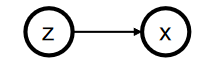
\includegraphics[width=.25\textwidth]{微信图片_20200302213857.png}
    \caption{GMM的概率图模型}
\end{figure}
GMM从几何角度来看,就是也就是多个高斯分布来取加权平均值。我们想将样本分成多少类,那么$Z$就有多少种可能,假设我们需要将其分成$N$类。那么$Z$是一个离散变量,$Z\in \{1,2,3,\cdots,N\}$,当$Z$取每次取不同的值时都对应着一个不同的高斯分布,公式化表达为:$P(x|z)\sim \mathcal{N}(\mu,\sigma^2)$。那么对于一个样本,我们可以计算出它属于每一个类别的不同的概率,从中选取概率最大的即可。GMM举例如下图所示:
\begin{figure}[H]
    \centering
    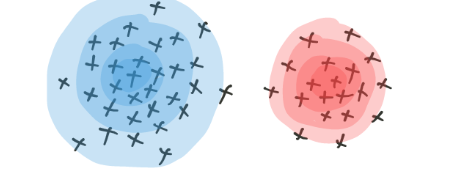
\includegraphics[width=.45\textwidth]{微信图片_20200302215950.png}
    \caption{GMM的概率图模型}
\end{figure}
GMM相关的具体知识,包括GMM的定义和EM算法进行求解等,请阅读小编之前写的“白板推导 高斯混合模型”。很明显,我们看到GMM的边界轮廓都是圆的,学术的讲就是“凸”(Convex)的。\textbf{这样的考虑忽略了数据之间的结构关系,主要考虑的是特征之间的相似度,而且是一种中心的距离方式。}而这时候我们需要引出另一种聚类算法的思路了,连通性(Connectivity)。

\subsection{连通性聚类(Connectivity)}
连通性聚类(Connectivity)算法的典型代表就是谱聚类(Spectral Clustering)。比如,下面的数据分布,很显然用Spectral Clustering的方法来聚类成如下的形式更加的合理。如下图所示。\textbf{很显然这是一个non-convex的聚类方式,更加注重的是数据分布之间的连通性,并且利用图结构考虑到了数据内部的结构性特点,目标是使不同的类别数据点分的越开越好,至于为什么?请接着往下看Spectral Clustering的模型描述}。
\begin{figure}[H]
    \centering
    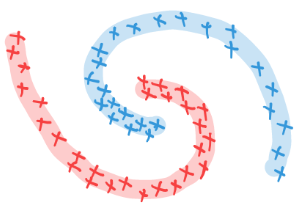
\includegraphics[width=.25\textwidth]{微信图片_20200302231505.png}
    \caption{Spectral Clustering示例}
    \label{fig:my_label_1}
\end{figure}
\subsection{小结}
聚合型聚类(Compactness)和连通性聚类(Connectivity)方法各有千秋。对于“凸”型形状,聚合型聚类(Compactness)更好一些,主要考虑的是特征之间的相似度。在复杂情况下,结合Kernel的做法可以简化计算,这个在“核技巧”那章有详细的说明。而连通性聚类(Connectivity)方法,主要考虑的是数据的结构上的特点,适合随意的形状。


\section{Spectral Clustering的模型表示}
\subsection{Spectral Clustering参数说明}
\textbf{Spectral Clustering的模型表示实现手段上是使用基于无向带权图的思想。}我们将所有的数据样本都分别当成无向图中的一个节点,我们假设概率图模型为:

$G=\{V,E\}$;

$V=\{1,2,3,\cdots,N\}$:无向图中每一个节点代表一个数据样本,图中有$N$个节点,代表有$N$个样本。

$X=\begin{bmatrix}x_1,x_2,\cdots,x_N\end{bmatrix}^T = \begin{bmatrix}x_1^T \\ x_2^T \\ \vdots \\ x_N^T\end{bmatrix}_{N\times p} $:代表有$N$个样本,每个样本都是$p$维的。而$V$中的$i$就对应着$x_i$,表示第$i$个样本。

$E:[w_{ij}]_{n\times n}$:这个被称为相似度矩阵,也就是用来表示样本与样本之间的权重。只有点与点之间存在边,才有权重,否则为0。比如如下图所示的一个概率图结构:
\begin{figure}[H]
    \centering
    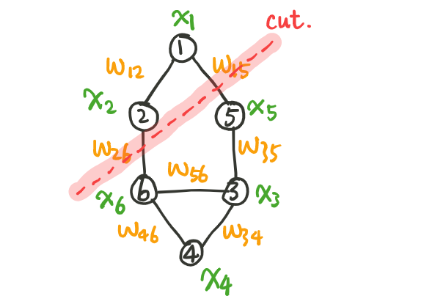
\includegraphics[width=.4\textwidth]{微信图片_20200303131334.png}
    \caption{Spectral Clustering示例}
\end{figure}
其中:
$$
w_{ij} = 
\left\{
\begin{array}{ll}
      k(x_i,x_j) = \exp \left\{ -\frac{||x_i-x_j||^2_2}{2\sigma^2} \right\} &(i,j)\in E \\
      0 & (i,j)\neq E \\
\end{array}
\right.
$$
其实在概率图中体现就是,有连接的地方就有权重,没有连接的地方就没有权重。所以,这样就可以反映数据的条件独立性和结构特点,只有某些点之间才有联系,而不是像GMM那样,默认所有点之间都有联系。

\subsection{Spectral Clustering优化目标}
定义:$A\subset V$,$B\subset V$,$A \cap B=\varnothing$,$W(A,B)=\sum_{i\in A}\sum_{j\in B}w_{ij}$。这个公式描述的是将节点分成两份,每个节点都只能属于其中一类,他们之间的距离定义为,一个集合中的每一个节点,分别到另一个集合中的所有节点的相似度的和。

如果,想将节点分解成$K$类,那么公式化描述如下所示:
\begin{equation}
    \begin{split}
        & \mathrm{cut}(V) = \mathrm{cut}(A_1,A_2,\cdots,A_K) \\
        & \left\{
        \begin{array}{ll}
        V = \bigcup_{k=1}^K A_k & \\
        A_i \cap A_j = \varnothing, \ \forall i,j\in \{ 1,2,\cdots,K \}& \\
        \end{array}
\right.
    \end{split}
\end{equation}

并且令:
\begin{equation}
    \mathrm{cut}(V) = \sum_{k=1}^K W(A_k,\Bar{A}_k) = \sum_{k=1}^K \sum_{p\in A_k} \sum_{q\notin A_k} w_{pq}
\end{equation}
其中,$\Bar{A}_k$表示出了$A_k$以外的所有子集构成的集合。那么这个公式的意思就是,每个集合中的所有点,分别到其他集合中的所有点的相似度的和。那么我们的目标函数,首先可以定义为最小化这个cut函数。因为\textbf{该值与聚类的目标一致,即每个子图内部的连接很强,而子图之间的连接很弱,换一种语言来表述就是同一个子图内的样本相似,不同子图之间的样本不相似。}即为:
\begin{equation}
    \min_{\{A_k\}_{i=k}^K}\mathrm{cut}(V)
\end{equation}
其实,也就是要将$V$划分$K$类,使得$\mathrm{cut}$函数值最小,实际上就是一个组合优化问题。

\subsection{Spectral Clustering优化目标改进}
但是,我们观察上述的式子,实际上是有不妥的地方的。比如,图四中,有一类为2个节点,另一类为4个节点。\textbf{但直接通过最小化这个值实现聚类还有问题,它没有考虑子图规模对代价函数的影响,使得这个指标最小的切分方案不一定就是最优切割。}因此需要对代价函数进行归一化。

第一种最简单的思路,既然我们需要考虑子图的规模,就是除以集合中点的个数(优化类别的平均代价之和),即为:
\begin{equation}
    \mathrm{cut}(V) = \sum_{k=1}^K \frac{W(A_k,\Bar{A}_k)}{|A_k|}
\end{equation}

但是,这样做仍然不妥,因为这样即使考虑了集合中点的个数。子图的复杂度还需要考虑子图中节点的连接情况,而不是仅仅考虑子图的个数即可。考虑子图中的连接也侧面包含了子图的节点个数所带来的复杂度。为了量化连接情况,这里引入一个概念为“度”:这是离散数学中的定义,有向图中分“出度”和“入度”,其实很简单“出度”就是这个节点指向了几个节点,“入度”就是有几个节点指向这个节点。无向图中我们只用度的概念。

而在带权无向图中,一个节点的度即为与这个节点连接的所有的边的权重和。利用度作为归一化因子就比较全面的考虑了子图的复杂度了。
\begin{equation}
    \mathrm{degree(A_k)} = \sum_{i\in A_k} d_i,\quad d_i = \sum_{j=1}^N w_{ij}
\end{equation}
那么就得到了,最终的优化目标为:
\begin{equation}
    \min_{\{A_k\}_{k=1}^K} \mathrm{Ncut}(V) = \sum_{k=1}^K\frac{ W(A_k,\Bar{A}_k)}{\sum_{i\in A_k} d_i} ,\quad d_i = \sum_{j=1}^N w_{ij}
\end{equation}

\subsection{小结}
本小节我们定义了谱聚类的目标函数,该函数值反映的聚类的目标为,同一个子图内的样本相似,不同子图之间的样本不相似。因为需要考虑子图的复杂度,我们对目标函数进行了优化。考虑子图中的连接情况,用“度”的概念来定义子图的复杂度。从而通过引入“度”来表示对子图复杂度的影响,来优化目标函数。

\section{目标函数的矩阵表达形式}
通过上一小节,我们得到了算法的目标函数为:
\begin{equation}
    \{ \hat{A}_k \}_{k=1}^K = \arg\min_{\{A_k\}_{k=1}^K} \sum_{k=1}^K\frac{ W(A_k,\Bar{A}_k)}{\sum_{i\in A_k} \sum_{j=1}^N w_{ij}}  
\end{equation}
因为求解的过程中,连加符号并不方便进行各种运算操作。所以,我们要把目标函数转换为矩阵形式,从而方便计算。首先,这个$\{ \hat{A}_k \}_{k=1}^K$(表示的是将所有的点进行划分后的结果)看着就不好进行运算,所以第一步想办法把这个变成矩阵化表示。
\subsection{指示向量(Indicator vector)}
令:
$$
\left\{
\begin{array}{ll}
      y_i \in \{0,1\}^K & \\
      \sum_{j=1}^K y_{ij} = 1 & \\
\end{array}
\right.
$$
这个公式想要表达的意思为,$y_i$是一个$K$维向量,每一个维度的值要么是0,要么是1。$y_{ij} = 1$表示第$i$个样本属于第$j$个类别,而每个样本只能属于一个类别,所以$\sum_{j=1}^K y_{ij} = 1$,$1\leq i \leq N$,$1\leq j \leq K$。那么使用Indicator vector后,目标函数为:
$$
Y = (y_1,y_2,\cdots,y_N)^T_{N\times K}
$$
$$
\hat{Y} = \arg\min_{Y} \sum_{k=1}^K \frac{ W(A_k,\Bar{A}_k)}{\sum_{i\in A_k} \sum_{j=1}^N w_{ij}} 
$$
利用指示函数将$\{ \hat{A}_k \}_{k=1}^K$变成矩阵以后,下一步目标就是将后面那一坨改写成矩阵形式。
\subsection{对角矩阵}
在使用只是向量后,我们成功的将目标函数化简成了:
\begin{equation}
    \begin{split}
        & Y = (y_1,y_2,\cdots,y_N)^T_{N\times K} \\
        & \hat{Y} = \arg\min_{Y} \sum_{k=1}^K \frac{ W(A_k,\Bar{A}_k)}{\sum_{i\in A_k} d_i },\quad d_i = \sum_{j=1}^N w_{ij} 
    \end{split}
\end{equation}
我们的下一步目标就是想想如何将$\sum_{k=1}^K \frac{ W(A_k,\Bar{A}_k)}{\sum_{i\in A_k} d_i } $表达成矩阵形式。\textbf{求和符号可以被我们写做对角矩阵的trace};所以有:
\begin{equation}
\begin{split}
    \mathrm{Ncut}(V) = & \sum_{k=1}^K \frac{ W(A_k,\Bar{A}_k)}{\sum_{i\in A_k} d_i } = 
    \mathrm{tr}
    \left(
    \begin{bmatrix}
    \frac{ W(A_1,\Bar{A}_1)}{\sum_{i\in A_1} d_i } & 0 & \cdots & 0 \\
    0 & \frac{ W(A_2,\Bar{A}_2)}{\sum_{i\in A_2} d_i } &   \cdots & 0 \\
    \vdots & \vdots & \ddots & \vdots \\
    0 & 0  &   \cdots & \frac{ W(A_K,\Bar{A}_K)}{\sum_{i\in A_K} d_i } \\
    \end{bmatrix}_{K\times K} 
    \right) \\
    = & 
    \mathrm{tr}
    \left(
    \underbrace{
    \begin{bmatrix}
    { W(A_1,\Bar{A}_1)} & 0 & \cdots & 0 \\
    0 &  W(A_2,\Bar{A}_2) &   \cdots & 0 \\
    \vdots & \vdots & \ddots & \vdots \\
    0 & 0  &   \cdots & { W(A_K,\Bar{A}_K)} \\
    \end{bmatrix}}_{O_{K\times K}}
    {\underbrace{\begin{bmatrix}
    {\sum_{i\in A_1} d_i } & 0 & \cdots & 0 \\
    0 & {\sum_{i\in A_2} d_i } &   \cdots & 0 \\
    \vdots & \vdots & \ddots & \vdots \\
    0 & 0  &   \cdots & {\sum_{i\in A_K} d_i } \\
    \end{bmatrix}}_{P_{K\times K}}}^{-1}
    \right)
    \\
    = & \mathrm{tr}(OP^{-1})
\end{split}
\end{equation}
其中,$O$和$P$都是对角矩阵。\textbf{首先我们需要明确一下,哪些变量是知道的,1. 相似度矩阵:$W=[w_{ij}]_{n\times n}$;2. 指示变量:$Y$($Y$每次都是已知的,我们的目标就是众多种可能性中,找使得目标函数最大的$Y$)。}{\color{red}所以,我们的目标是用$W$和$Y$来表示$O$和$P$。}

~\\

首先来看看如何表示$P$矩阵。

$\sum_{i\in A_k} d_i $代表的是,第$k$类集合中,所有的节点的度的和。而无向图中的度就是一个节点与其他所有节点所连接的边的权重之和。而$W=[w_{ij}]_{n\times n}$矩阵中$w_{ij}$代表第$i$个节点与第$j$个节点的权值,所以$W$矩阵\textbf{,第$i$行的所有值的和正好就是第$i$个节点与其他所有节点连接的边的权重之和。}

所以,计算方法就是将$W$矩阵,每一行的所有值都相加。度的对角矩阵可以描述为:
\begin{equation}
    D = \mathrm{diag}\left[W
    \begin{bmatrix}
    1 \\ 1 \\ \vdots \\ 1 
    \end{bmatrix}_{N\times 1}\right]
    = \begin{bmatrix}
    d_1 & & & \\
     & d_2 & & \\
     & & \ddots & \\
     & & & d_N \\
    \end{bmatrix}
\end{equation}


那么,下一步目标就是将这些度分别按划分的类别进行求和,也就是比如$A_1=\{1,2,5\}$,那么就要把第1,2,5三个节点的度加在一起。那么,应该如何去实现呢?

$Y$矩阵是$N\times K$维的,行代表节点标号,列代表属于的类别。那么,$y_{ij} = 1$表示第$i$个样本属于第$j$个类别。那么,我们从$Y$中取出第$i$行向量($1\times K$)来,那么通过这一行向量,根据第几列的值等于1,我们可以看出这个样本属于第几类。假设这个行向量第$j$列等于0;那么$y_i^Ty_i$结果为:
\begin{equation}
y_i^Ty_i=  
    \begin{bmatrix}
    0 \\ 0\\ \cdots\\y_{ij}=1\\ \cdots\\0 \\
    \end{bmatrix}
     \begin{bmatrix}
    0 & 0& \cdots&y_{ij}=1&\cdots&0 \\
    \end{bmatrix}
    =
    \begin{bmatrix}
    0 & \cdots & 0 &\cdots & 0 \\
    \vdots & \ddots & \vdots &\ddots & \vdots \\
     0 & \cdots & y_{jj}=1 &\cdots & 0 \\
     \vdots & \ddots & \vdots &\ddots & \vdots \\
     0 & \cdots & 0 &\cdots & 0 \\
    \end{bmatrix}
\end{equation}

那么,很显然$y_i^T D y_i$求得的是一个$K\times K$的矩阵,而这个矩阵中只有一个元素不为零,其他的元素都为零。如果$y_i$样本属于第$k$类,那么这个元素的位置为第$k$行,第$k$列,元素的值为$d_i$。通过这样的运算,\textbf{我们成功的实现了,如果第$i$个样本属于第$k$类,就将这个样本的度$d_i$,放在了$K \times K$的矩阵第$k$行,第$k$列的位置。而且这个矩阵一定是对角矩阵。}

有$N$个样本就算有$N$个这样的矩阵,把这$N$个矩阵加起来就实现了将所有的$d_i$按所属的类别求和的工作。也就是:
\begin{equation}
    \sum_{i=1}^N y_i d_{i} y_i^T = Y^TDY 
\end{equation}

这个式子的计算可以这样考虑:先算$y_i d_i$,也就是$(y_1d_1,y_2d_2,\cdots,y_Nd_N)$,可以表示成:
\begin{equation}
    (y_1,y_2,\cdots,y_N)diag(d_1,d_2,\cdots,d_N)
\end{equation}


所以,我们就得到了用$Y$和$W$对$P$矩阵的进行表达的形式为:
\begin{equation}
    P = Y^T\mathrm{diag}(W\cdot \mathbf{1_N})Y
\end{equation}
其中,$\mathbf{1_N}$元素全为1的$N\times1$维向量。

\subsection{拉普拉斯矩阵(Lapalacian Matrix)}
成功将$P$表示以后,下一步目标则是想办法表示$O$矩阵。
\begin{equation}
    \begin{bmatrix}
    { W(A_1,\Bar{A}_1)} & 0 & \cdots & 0 \\
    0 &  W(A_2,\Bar{A}_2) &   \cdots & 0 \\
    \vdots & \vdots & \ddots & \vdots \\
    0 & 0  &   \cdots & { W(A_K,\Bar{A}_K)} \\
    \end{bmatrix}_{K\times K}
\end{equation}
而$\Bar{A}_i$代表的是,整个样本集中去除$A_i$中的样本后的所有样本。那么,可以做下列变换:
\begin{equation}
    W(A_k,\Bar{A}_k) = W(A_k,V) - W(A_k,A_k)
\end{equation}

根据$W(\cdot)$函数的定义,$W(A,B)$函数表示的是$A$中所有点分别到$B$中所有点的相似度的和,即为:
\begin{equation}
    W(A_i,A_j) = \sum_{p\in A_i} \sum_{q\notin A_j} w_{pq}
\end{equation}
所以,$ W(A_k,V) = \sum_{i\in A_k} d_i$,$W(A_k,A_k) = \sum_{i\in A_k} \sum_{j\in A_k} w_{ij}$。而$W(A_k,V) = \sum_{i\in A_k} d_i$是$ Y^T\mathrm{diag}(W\cdot 1_N)Y$这一对角矩阵对角上的一个元素,下一步只要想办法表达$W(A_k,A_k) = \sum_{i\in A_k} \sum_{j\in A_k} w_{ij}$即可。我们的目标是求解同一个类别中,任意两个不同的样本之间的相似度。这其实和上一个求$P$的问题非常的类似,那么首先来看看$Y^TWY$会等于什么,因为$Y = (y_1,y_2,\cdots,y_N)^T_{N\times K}$,所以:
\begin{equation}
    \begin{split}
        Y^TWY = &
        \begin{bmatrix}
        y_1 & y_2 & \cdots & y_N \\
        \end{bmatrix}
        \begin{bmatrix}
        w_{11} & w_{12} & \cdots & w_{1N} \\
        w_{21} & w_{22} & \cdots & w_{2N} \\
        \vdots & \vdots & \ddots & \vdots \\
        w_{N1} & w_{N2} & \cdots & w_{NN} \\
        \end{bmatrix}
        \begin{bmatrix}
        y_1^T \\ y_2^T \\ \vdots \\ y_N^T \\
        \end{bmatrix} \\
        = & 
        \begin{bmatrix}
        \sum_{i=1}^N y_iw_{i1} & \cdots & \sum_{i=1}^N y_iw_{iN}
        \end{bmatrix}
        \begin{bmatrix}
        y_1^T \\ y_2^T \\ \vdots \\ y_N^T \\
        \end{bmatrix} \\
        = & \sum_{j=1}^N \sum_{i=1}^N y_iw_{ij}y_j^T
    \end{split}
\end{equation}
有因为$w_{ij}$是一个一维实数,所以,$Y^TWY = \sum_{j=1}^N \sum_{i=1}^N y_iw_{ij}y_j^T = \sum_{j=1}^N \sum_{i=1}^N y_iy_j^Tw_{ij}$。那么,我们考虑一下$y_iy_j^T$等于什么。$y_i$表示的是一个样本属于第几类,那么$y_i\in A_p$,$y_i\in A_q$,则$y_iy_j^T$得到的矩阵中第$i$行,第$j$列的元素值为1,其余的全部为0。所以:
\begin{equation}
    Y^TWY = \sum_{j=1}^N \sum_{i=1}^N y_iw_{ij}y_j^T = 
    \begin{bmatrix}
    \sum_{i\in A_1}\sum_{j \in A_1} w_{ij} & \sum_{i\in A_1}\sum_{j \in A_2} w_{ij} & \cdots & \sum_{i\in A_1}\sum_{j \in A_k} w_{ij} \\
    \sum_{i\in A_2}\sum_{j \in A_1} w_{ij} & \sum_{i\in A_2}\sum_{j \in A_2} w_{ij} & \cdots & \sum_{i\in A_2}\sum_{j \in A_k} w_{ij} \\
    \vdots & \vdots & \ddots & \vdots \\
    \sum_{i\in A_k}\sum_{j \in A_1} w_{ij} & \sum_{i\in A_k}\sum_{j \in A_2} w_{ij} & \cdots & \sum_{i\in A_k}\sum_{j \in A_k} w_{ij} \\
    \end{bmatrix}
\end{equation}

而:
\begin{equation}
\begin{split}
    \begin{bmatrix}
    { W(A_1,\Bar{A}_1)} & 0 & \cdots & 0 \\
    0 &  W(A_2,\Bar{A}_2) &   \cdots & 0 \\
    \vdots & \vdots & \ddots & \vdots \\
    0 & 0  &   \cdots & { W(A_K,\Bar{A}_K)} \\
    \end{bmatrix} = & 
    \begin{bmatrix}
    { W(A_1,V)} & 0 & \cdots & 0 \\
    0 &  W(A_2,V) &   \cdots & 0 \\
    \vdots & \vdots & \ddots & \vdots \\
    0 & 0  &   \cdots & { W(A_K,V)} \\
    \end{bmatrix} \\
     & -
    \begin{bmatrix}
    { W(A_1,A_1)} & 0 & \cdots & 0 \\
    0 &  W(A_2,A_2) &   \cdots & 0 \\
    \vdots & \vdots & \ddots & \vdots \\
    0 & 0  &   \cdots & { W(A_K,A_K)} \\
    \end{bmatrix} \\
    = &  Y^TDY  - \begin{bmatrix}
    { W(A_1,A_1)} & 0 & \cdots & 0 \\
    0 &  W(A_2,A_2) &   \cdots & 0 \\
    \vdots & \vdots & \ddots & \vdots \\
    0 & 0  &   \cdots & { W(A_K,A_K)} \\
    \end{bmatrix} 
\end{split}
\end{equation}

我们关注的是trace,所以只要对角线上的元素是一样的就可以了。令$O' = Y^TDY - Y^TWY$,而$\mathrm{tr}(O'P^{-1})=\mathrm{tr}(OP^{-1})$,因为$O'$和$O$对角线上的元素都是一样的。所以,最终我们把Ncut目标函数化简成了矩阵的表达形式为:
\begin{equation}
    \hat{Y} = \arg\min_Y \mathrm{tr}\left\{ Y^T(D-W)Y\cdot (Y^TDY)^{-1} \right\},\quad D = \mathrm{diag}(W\cdot 1_N)
\end{equation}

其中$(D-W)$被称为拉普拉斯矩阵(Lapalacian Matrix)。最终,我们成功的用已知的$Y$和$W$来完成了对目标函数Ncut的矩阵化。有关拉普拉斯矩阵的性质,后面会讲到,这是图中一个很重要的矩阵,感兴趣的同学也可以看看https://zhuanlan.zhihu.com/p/67336297,对拉普拉斯矩阵和拉普拉斯算子的详细介绍。

\subsection{小结}
这一小节中,我们主要的工作就是将目标函数“Ncut函数”化简为矩阵形式。首先我们用指示向量来表示样本所属的类别。然后利用指示函数($Y$)和相似度矩阵($W$)来对Ncut函数进行表示。其实我觉得这里就可以看成是特征值分解后的结果。最终的变换结果和拉普拉斯矩阵有关系,有关拉普拉斯矩阵的详细内容有兴趣的同学可以自行查阅。

\section{总结(Conclusion)}
这节主要讲述的是谱聚类算法,首先讲述了两种不同的聚类思路,一种就是聚合型聚类(Compactness),另一种是连通性聚类(Connectivity)算法。聚合性聚类更多的考虑是所有样本之间都是一视同仁的,根据特征的相似度来聚类。连通性聚类更多的考虑的是数据之间的分布结构,不同的数据之间可以有关系也可以没有关系,这样便于人们引入对数据的侧重点的分析,有点条件独立的意思在里面。而连通性聚类(Connectivity)算法需要借助图结构来实现。我们介绍了谱聚类算法的目标函数,然后对目标函数进行了优化,为了计算的方便,又描述了目标函数的矩阵表达形式。整个过程比较流程。
\end{document}
